\index{类型!族的|(}%
\index{运输|(defstyle}%
因为在类型伦中\emph{依赖类型}函数是必须的, 所以也需要依赖类型版本的\cref{lem:map}. 然而这并不简单, 因为如果 $f:\prd{x:A} B(x)$ 和 $p:x=y$, 那么 $f(x):B(x)$ 和 $f(y):B(y)$ 是不同类型的元素, 所以\emph{事实上}, 我们甚至不能询问他们是否相等. 缺少的部分是, $p$ 本身给了一个关联 $B(x)$ 和 $B(y)$ 的方式.

我们已经在\autoref{sec:identity-types}见过了, 它被称为``恒等的不可区分性''. \index{恒等的不可区分性}%
现在介绍它的一个不同的名字和符号, 我们从现在开始使用.

\begin{lem}[运输]\label{lem:transport}
提供 $A$ 上的类型族 $P$ 和 $p:\id[A]xy$.
则有一个函数 $\transf{p}:P(x)\to P(y)$.
\end{lem}

\begin{proof}[第一个证明]
令$D:\prd{x,y:A} (\id{x}{y}) \to \type$ 为一个类型族, 其定义为
\[D(x,y,p)\defeq P(x)\to P(y).\]
那么有函数
\begin{equation*}
d\defeq\lam{x} \idfunc[P(x)]:\prd{x:A} D(x,x,\refl{x}),
\end{equation*}
于是归纳原理给出对于 $p:x= y$ 有 $\indid{A}(D,d,x,y,p):P(x)\to P(y)$, 也就是 $\transf p$ 的定义.
\end{proof}

\begin{proof}[第二个证明]
通过归纳, 足以认为 $p$ 是 $\refl x$.
在这个情况下, 可以令 $\transf{(\refl x)}:P(x)\to P(x)$ 为恒等函数.
\end{proof}

有时, 在运输符号上, 有必要把类型族 $P$ 用符号表示. 这种情况下, 可以写作 \[\transfib P p \blank : P(x) \to P(y).\]

回顾 $A$ 上的类型族 $P$ 可以被视作 $A$ 的元素的性质, 当 $x$ 是 $A$ 的元素且 $P(x)$ 有居留元时, 这个性质成立. 然后运输定理表示 $P$ 的平等性, 从在种意义上, 如果 $x$ 等于 $y$, 那么当且仅当 $P(y)$ 成立时 $P(x)$ 成立. 实际上, 以后可以看到如果 $x=y$ 则实际上 $P(x)$ 和 $P(y)$ 是\emph{等价的}.

拓扑上, 运输定理可以被视为纤维中的``路径提升''操作. \index{纤维}%
\indexdef{总和!空间}%
可以这么认为, 类型族 $P:A\to \type$ 是一个底空间 $A$的 \emph{纤维结构}, 其中 $P(x)$ 是 $x$ 上的纤维, $\sm{x:A}P(x)$ 是纤维结构的\define{群空间}, 和第一投影 $\sm{x:A}P(x)\to A$. 纤维结构所定义的性质是给定一个底空间 $A$ 上的路径 $p:x=y$, 和经过 $x$ 的纤维的一个点 $u:P(x)$, 可以提升路径 $p$ 到起始于 $u$ 的群空间的路径(该提升可以连续完成). 点 $\trans p u$ 可以被认为是提升路径的另一个端点. 还可以在类型中定义路径本身:

\begin{lem}[路径提升性质]\label{thm:path-lifting}
\indexdef{路径!提升}%
\indexdef{提升!路径}%
令 $P:A\to\type$ 为一个经过 $A$ 的类型族, 并假设对于一些 $x:A$ 有 $u:P(x)$.
然后对于任何 $p:x=y$, 有
\begin{equation*}
\mathsf{lift}(u,p):(x,u)=(y,\trans{p}{u})
\end{equation*}
在 $\sm{x:A}P(x)$, 于是 $\ap{\proj1}{\mathsf{lift}(u,p)} = p$.
\end{lem}
\begin{proof}
留给读者.
在\cref{sec:compute-sigma}会证明更普遍的定理 .
\end{proof}

在经典同伦论, 纤维结构被定义为映射, \emph{发生于}路径的提升; 相比之下, 我们刚刚展示了在类型伦中, 每个类型族都是\emph{特殊的} ``路径提升函数''. 这符合构造主义数学的哲学, 只有展示它, 才能说某个事物存在. \index{类型伦中函数的连续性@类型伦中函数的``连续性''}%
因为我们已经看到, 类型伦中所有函数都是``连续的'', 因此确保了路径提升具备良好的``连续性''.

\begin{rmk}
景观我们可能认为类型族 $P:A\to \type$ 就像一个纤维结构一样, 但广泛地说``纤维 $P:A\to\type$'' 并不是一个好主意, 因为这听起来像是在说基于底 $\type$ 和群空间 $A$的纤维结构.
重复一遍, 当一个类型族 $P:A\to \type$ 被视为是一个纤维结构时, 它的底是 $A$ 而群空间是 $\sm{x:A} P(x)$.

在讨论类型族时, 可能还会使用其它拓扑术语.
例如, 可能会把依赖函数 $f:\prd{x:A} P(x)$ 称作纤维结构 $P$ 的\define{截面}
\indexdef{截面!类型族的}%
, 而我们说一些事物发生了\define{纤维化}
\indexdef{纤维化}%
如果每个 $P(x)$ 都出现这种情况.
例如, 一个截面 $f:\prd{x:A} P(x)$ 展示了 $P$ 是 ``纤维化居留的''.
\end{rmk}

\index{函数!依赖|(}
现在我们可以证明\cref{lem:map}的依赖版本了. 拓扑的直觉是给定 $f:\prd{x:A} P(x)$ 和一个路径 $p:\id[A]xy$, 可以应用 $f$ 到 $p$ 并得到 $P$  的群空间中的一个路径, 它``位于'' $p$ 下方.

\begin{center}
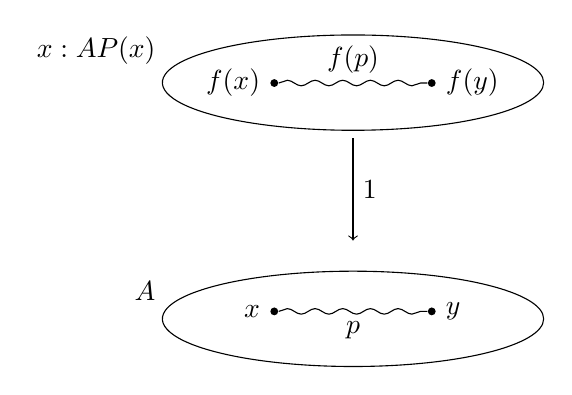
\begin{tikzpicture}[yscale=.5,xscale=2]
\draw (0,0) arc (-90:170:8ex) node[anchor=south east] {$A$} arc (170:270:8ex);
\draw (0,6) arc (-90:170:8ex) node[anchor=south east] {$\sm{x:A} P(x)$} arc (170:270:8ex);
\draw[->] (0,5.8) -- node[auto] {$\proj1$} (0,3.2);
\node[circle,fill,inner sep=1pt,label=left:{$x$}] (b1) at (-.5,1.4) {};
\node[circle,fill,inner sep=1pt,label=right:{$y$}] (b2) at (.5,1.4) {};
\draw[decorate,decoration={snake,amplitude=1}] (b1) -- node[auto,swap] {$p$} (b2);
\node[circle,fill,inner sep=1pt,label=left:{$f(x)$}] (b1) at (-.5,7.2) {};
\node[circle,fill,inner sep=1pt,label=right:{$f(y)$}] (b2) at (.5,7.2) {};
\draw[decorate,decoration={snake,amplitude=1}] (b1) -- node[auto] {$f(p)$} (b2);
\end{tikzpicture}
\end{center}

从\cref{lem:map}\emph{可以}得到这样的东西. Given $f:\prd{x:A} P(x)$, we can define a non-dependent function $f':A\to \sm{x:A} P(x)$ by setting $f'(x)\defeq (x,f(x))$, and then consider $\ap{f'}{p} : f'(x) = f'(y)$. Since $\proj1 \circ f' \jdeq \idfunc[A]$, by \cref{lem:ap-functor} we have $\ap{\proj1}{\ap{f'}{p}} = p$; thus $\ap{f'}{p}$ does ``lie over'' $p$ in this sense. However, it is not obvious from the \emph{type} of $\ap{f'}{p}$ that it lies over any specific path in $A$ (in this case, $p$), which is sometimes important.

The solution is to use the transport lemma. By \cref{thm:path-lifting} we have a canonical path $\mathsf{lift}(u,p)$ from $(x,u)$ to $(y,\trans p u)$ which lies over $p$. Thus, any path from $u:P(x)$ to $v:P(y)$ lying over $p$ should factor through $\mathsf{lift}(u,p)$, essentially uniquely, by a path from $\trans p u$ to $v$ lying entirely in the fiber $P(y)$. Thus, up to equivalence, it makes sense to define ``a path from $u$ to $v$ lying over $p:x=y$'' to mean a path $\trans p u = v$ in $P(y)$. And, indeed, we can show that dependent functions produce such paths.

\begin{lem}[Dependent map]\label{lem:mapdep}
\indexdef{application!of dependent function to a path}%
\indexdef{path!application of a dependent function to}%
\indexdef{function!dependent!application to a path of}%
\indexdef{action!of a dependent function on a path}%
Suppose $f:\prd{x: A} P(x)$; then we have a map
\[\apdfunc f : \prd{p:x=y}\big(\id[P(y)]{\trans p{f(x)}}{f(y)}\big).\]
\end{lem}

\begin{proof}[第一个证明]
令$D:\prd{x,y:A} (\id{x}{y}) \to \type$ 为一个类型族, 其定义为
\begin{equation*}
D(x,y,p)\defeq \trans p {f(x)}= f(y).
\end{equation*}
Then $D(x,x,\refl{x})$ is $\trans{(\refl{x})}{f(x)}= f(x)$.
But since $\trans{(\refl{x})}{f(x)}\jdeq f(x)$, we get that $D(x,x,\refl{x})\jdeq (f(x)= f(x))$.
Thus, we find the function
\begin{equation*}
d\defeq\lam{x} \refl{f(x)}:\prd{x:A} D(x,x,\refl{x})
\end{equation*}
and now path induction gives us $\apdfunc f(p):\trans p{f(x)}= f(y)$ for each $p:x= y$.
\end{proof}

\begin{proof}[第二个证明]
通过归纳, 足以认为 $p$ 是 $\refl x$.
But in this case, the desired equation is $\trans{(\refl{x})}{f(x)}= f(x)$, which holds judgmentally.
\end{proof}

We will refer generally to paths which ``lie over other paths'' in this sense as \emph{dependent paths}. \indexsee{dependent!path}{path, dependent}%
\index{path!dependent}%
They will play an increasingly important role starting in \cref{cha:hits}. In \cref{sec:computational} we will see that for a few particular kinds of type families, there are equivalent ways to represent the notion of dependent paths that are sometimes more convenient.

Now recall from \cref{sec:pi-types} that a non-dependently typed function $f:A\to B$ is just the special case of a dependently typed function $f:\prd{x:A} P(x)$ when $P$ is a constant type family, $P(x) \defeq B$. In this case, $\apdfunc{f}$ and $\apfunc{f}$ are closely related, because of the following lemma:

\begin{lem}\label{thm:trans-trivial}
If $P:A\to\type$ is defined by $P(x) \defeq B$ for a fixed $B:\type$, then for any $x,y:A$ and $p:x=y$ and $b:B$ we have a path
\[ \transconst Bpb : \transfib P p b = b. \]
\end{lem}
\begin{proof}[第一个证明]
Fix a $b:B$, and let $D:\prd{x,y:A} (\id{x}{y}) \to \type$ be the type family defined by
\[ D(x,y,p) \defeq (\transfib P p b = b). \]
Then $D(x,x,\refl x)$ is $(\transfib P{\refl{x}}{b} = b)$, which is judgmentally equal to $(b=b)$ by the computation rule for transporting.
Thus, we have the function
\[ d \defeq \lam{x} \refl{b} : \prd{x:A} D(x,x,\refl x). \]
Now path induction gives us an element of
\narrowequation{
\prd{x,y:A}{p:x=y}(\transfib P p b = b),}
as desired.
\end{proof}
\begin{proof}[第二个证明]
By induction, it suffices to assume $y$ is $x$ and $p$ is $\refl x$.
But $\transfib P {\refl x} b \jdeq b$, so in this case what we have to prove is $b=b$, and we have $\refl{b}$ for this.
\end{proof}

Thus, for any $x,y:A$ and $p:x=y$ and $f:A\to B$, by concatenating with $\transconst Bp{f(x)}$ and its inverse, respectively, we obtain functions \begin{align}
\big(f(x) = f(y)\big) &\to \big(\trans{p}{f(x)} = f(y)\big)\label{eq:ap-to-apd}
\qquad\text{and} \\
\big(\trans{p}{f(x)} = f(y)\big) &\to \big(f(x) = f(y)\big).\label{eq:apd-to-ap}
\end{align}
In fact, these functions are inverse equivalences (in the sense to be introduced in \cref{sec:basics-equivalences}), and they relate $\apfunc f (p)$ to $\apdfunc f (p)$.

\begin{lem}\label{thm:apd-const}
For $f:A\to B$ and $p:\id[A]xy$, we have
\[ \apdfunc f(p) = \transconst B p{f(x)} \ct \apfunc f (p). \]
\end{lem}
\begin{proof}[第一个证明]
Let $D:\prd{x,y:A} (\id xy) \to \type$ be the type family defined by
\[ D(x,y,p) \defeq \big(\apdfunc f (p) = \transconst Bp{f(x)} \ct \apfunc f (p)\big). \]
Thus, we have
\[D(x,x,\refl x) \jdeq \big(\apdfunc f (\refl x) = \transconst B{\refl x}{f(x)} \ct \apfunc f ({\refl x})\big).\]
But by definition, all three paths appearing in this type are $\refl{f(x)}$, so we have
\[ \refl{\refl{f(x)}} : D(x,x,\refl x). \]
Thus, path induction gives us an element of $\prd{x,y:A}{p:x=y} D(x,y,p)$, which is what we wanted.
\end{proof}
\begin{proof}[第二个证明]
By induction, it suffices to assume $y$ is $x$ and $p$ is $\refl x$.
In this case, what we have to prove is $\refl{f(x)} = \refl{f(x)} \ct \refl{f(x)}$, which is true judgmentally.
\end{proof}

Because the types of $\apdfunc{f}$ and $\apfunc{f}$ are different, it is often clearer to use different notations for them. % We may sometimes use a notation $\apd f p$ for $\apdfunc{f}(p)$, which is similar to the notation $\ap f p$ for $\apfunc{f}(p)$.


\index{function!dependent|)}%

At this point, we hope the reader is starting to get a feel for proofs by induction on identity types. From now on we stop giving both styles of proofs, allowing ourselves to use whatever is most clear and convenient (and often the second, more concise one). Here are a few other useful lemmas about transport; we leave it to the reader to give the proofs (in either style).

\begin{lem}\label{thm:transport-concat}
Given $P:A\to\type$ with $p:\id[A]xy$ and $q:\id[A]yz$ while $u:P(x)$, we have
\[ \trans{q}{\trans{p}{u}} = \trans{(p\ct q)}{u}. \]
\end{lem}

\begin{lem}\label{thm:transport-compose}
For a function $f:A\to B$ and a type family $P:B\to\type$, and any $p:\id[A]xy$ and $u:P(f(x))$, we have
\[ \transfib{P\circ f}{p}{u} = \transfib{P}{\apfunc f(p)}{u}. \]
\end{lem}

\begin{lem}\label{thm:ap-transport}
For $P,Q:A\to \type$ and a family of functions $f:\prd{x:A} P(x)\to Q(x)$, and any $p:\id[A]xy$ and $u:P(x)$, we have
\[ \transfib{Q}{p}{f_x(u)} = f_y(\transfib{P}{p}{u}). \]
\end{lem}

\index{type!family of|)}%
\index{transport|)}